\section{Evaluation of Existing Methods}
\subsection{Baseline Considerations}
It should be recalled that the work of 
CodeMirage\cite{guo2025codemirage} was not only to 
provide a dataset, but also to perform tests on 
some of the methods present in the literature.

The methods tested by CodeMirage can be divided into 4 categories:
\begin{enumerate}
    \item \textbf{Zero-shot detectors}: 
    These are methods based on the computation of code-related metrics and do not require any training.
    \newline The advantage of these methods is that they are totally independent of any dataset 
    and therefore “immune” to the \textit{out-of-domain effect}. This characteristic is very useful 
    if the detection method must be per-formant in different domains. 
    \newline Unfortunately, these methods also turn out to be complicated to develop 
    because they require a deep analysis of every type of code generated by an LLM, 
    unless such characteristics exist and are detectable by a non-AI-based method. 
    \newline Moreover, it is essential to identify characteristics that depend intrinsically on the 
    architecture of LLMs and not on their training, otherwise these methods would 
    become even less reliable over time than machine-learning-based methods.

    
    \item \textbf{Embedding-based detectors}: 
    These methods consist of using an encoder-only transformer 
    (or one that can be used as such), trained on code and not 
    fine-tuned for the classification task, paired with a classifier 
    trained on a dataset of LLM and human code.
    \newline These methods always remain inferior to the performance achieved by the next category.
    
    \item \textbf{Fine-tuned detectors}: 
    Fine-tuned methods are like embedding methods, but during training they 
    also train the encoder-only. The difference between the various methods 
    lies only in the choice of the encoder-only model. They seem to be the 
    models that in general achieve the best performance but are also the most 
    affected overall by the out-of-domain effect.
    
    \item \textbf{Pretrained LLM with downstream detector}:
    The last category is a middle ground between the previous ones and seems to 
    suffer overall less from out-of-domain problems. This category statistically 
    analyses the output of an LLM to which the code has been provided via a prompt, 
    such as \texttt{“explain this code:\{code\}”}. Such statistical 
    features are used by a classifier to learn which ones identify 
    human code more and which ones identify 
    LLM code.
\end{enumerate}

\subsubsection{CodeMirage problems}

\begin{figure}[H]
    \centering
    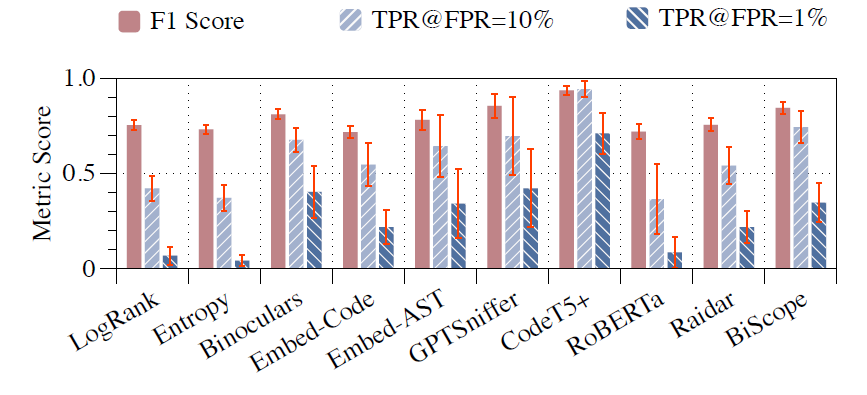
\includegraphics[width=1\textwidth]{img/CodeMirage/tests.png}
    \caption{CodeMirage's tests}
    \label{fig:CodeMirage-tests}
\end{figure}

The presented methods therefore fall into the previously described categories:
Zero-shot detectors: logRank\cite{gehrmann2019gltr}, entropy\cite{lavergne2008detecting}, 
binoculars\cite{hans2024spotting}.
Embedding-based detectors: Embed-Code, Embed-AST.
Fine-tuned detectors: GPTSniffer\cite{nguyen2024gptsniffer}, CodeT5+\cite{wang2023codet5+}, RoBERTa\cite{liu2019roberta}.
Pretrained LLM with downstream detector: Raidar\cite{mao2024raidar}, Bioscope \cite{guo2024biscope}.


Furthermore, these tests are not complete: 
recall that the CodeMirage dataset includes 
only code coming from GitHub and tends to be 
large. In addition, (more importantly), 
they never mention having removed comments in the code, 
which not infrequently (by analysing the dataset) appear 
to be extremely long and verbose. For this reason it is 
plausible that zero-shot methods designed for natural text 
apparently achieve good results on code as well 
(contrary to what many other works state: 
\textit{ zero-shot text detectors are ineffective in detecting code, 
likely due to the unique statistical properties found in code structures.}
\cite{yang2023zero}
).

It is important to make some clarifications: all the zero-shot 
methods presented were designed to analyze natural text which, 
as previously stated, is a process extremely different from 
analyzing code due to the naturally low next-token perplexity 
(a feature on which almost all zero-shot methods are based). 
The Embed-Code and Embed-AST methods are both based on 
CodeXEmbed-2B\cite{liu2024codexembed}, where in the first case code is provided and 
in the second case the AST obtained from code. GPTSniffer, 
CodeT5+, and RoBERTa are three methods that rely entirely on 
the GPTSniffer\cite{nguyen2024gptsniffer} technique and differ only by the encoder used. 
Finally, both Raidar and Bioscope are methods designed especially 
for natural text, but they seem to achieve good results on code as well.

For all the above reasons, it is justified not to stop at these tests but to pursue more in-depth analyses. In particular, additional methods not considered by CodeMirage and specifically designed for LLM code classification will be examined. Nevertheless, the CodeMirage results should not be ignored.

Key points: the method that appears to deliver the best performance 
is GPTSniffer with CodeT5+. BiScope also merits consideration. 
Rationale: CodeT5+ attains very high TPR at a 10\% 
FPR. However, these tests were run on a split of the 
CodeMirage dataset. Therefore, GPTSniffer with CodeT5+ 
was not evaluated out of domain, which is the main weakness 
of fine-tuned detectors, the category to which GPTSniffer with 
CodeT5+ belongs.

Similarly, BiScope belongs to the pretrained LLM with 
downstream detector category, which has fewer difficulties 
adapting to out-of-domain tests. It also achieves positive 
TPR at an FPR of 10\%. Therefore, GPTSniffer with 
CodeT5+ and BiScope will be considered the baselines 
for subsequent models.

It must be noted that CodeMirage has a major issue. In their work, 
it is never specified that the codes on which the methods are tested 
operate on clean code. By clean code it is meant code in which the 
natural-language sections (comments) have not been removed. 
This is actually fundamental for testing because it shows that the 
detection method does not rely on natural text but on code.
Moreover, the approach would become even less dataset-independent, 
since performance would risk varying extremely depending on the size 
of a code’s comment section.
A very strong and perhaps obvious statement can therefore be made: 
\textbf{any test on any dataset to which at least comment removal has not been 
applied is not to be considered valid for LLM code detection}.




\clearpage
\subsection{Methods to test}
An extensive survey of LLM code-detection methods 
in the literature was conducted. Many works were available 
only as preprints. Several seemingly promising papers could 
not be tested. For example, \cite{xu2025codevision} appears 
to leverage CNNs to analyse images of LLM- and human-written 
code for classification. Unfortunately, neither code nor 
pretrained models were accessible. Consequently, only a small 
set of other methods specifically designed for LLM code detection 
was evaluated.








%%%%%%%%%%%%%%%%%%%%%%%%%%%%%%%%%
\subsubsection{BiScope}
BiScope is a method designed for natural-text detection 
but was also tested by its authors on code detection.

\begin{figure}[H]
    \centering
    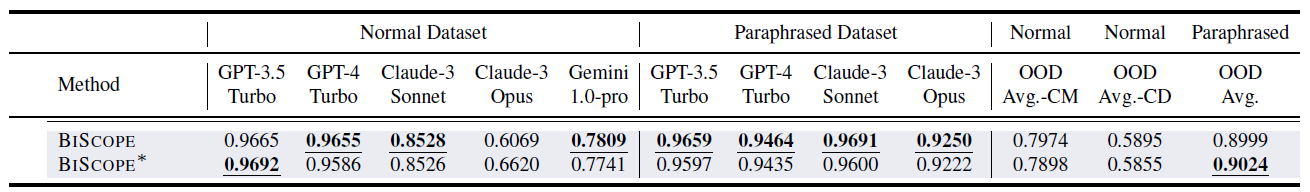
\includegraphics[width=1\textwidth]{img/BiScope/codetest.png}
    \caption{BiScope official code result from BiScope paper}
    \label{fig:BiScope official code result}
\end{figure}


Unlike methods that focus only on next-token prediction, 
BISCOPE evaluates text along two axes: next-token prediction 
and previous-token memorization.

\begin{figure}[H]
    \centering
    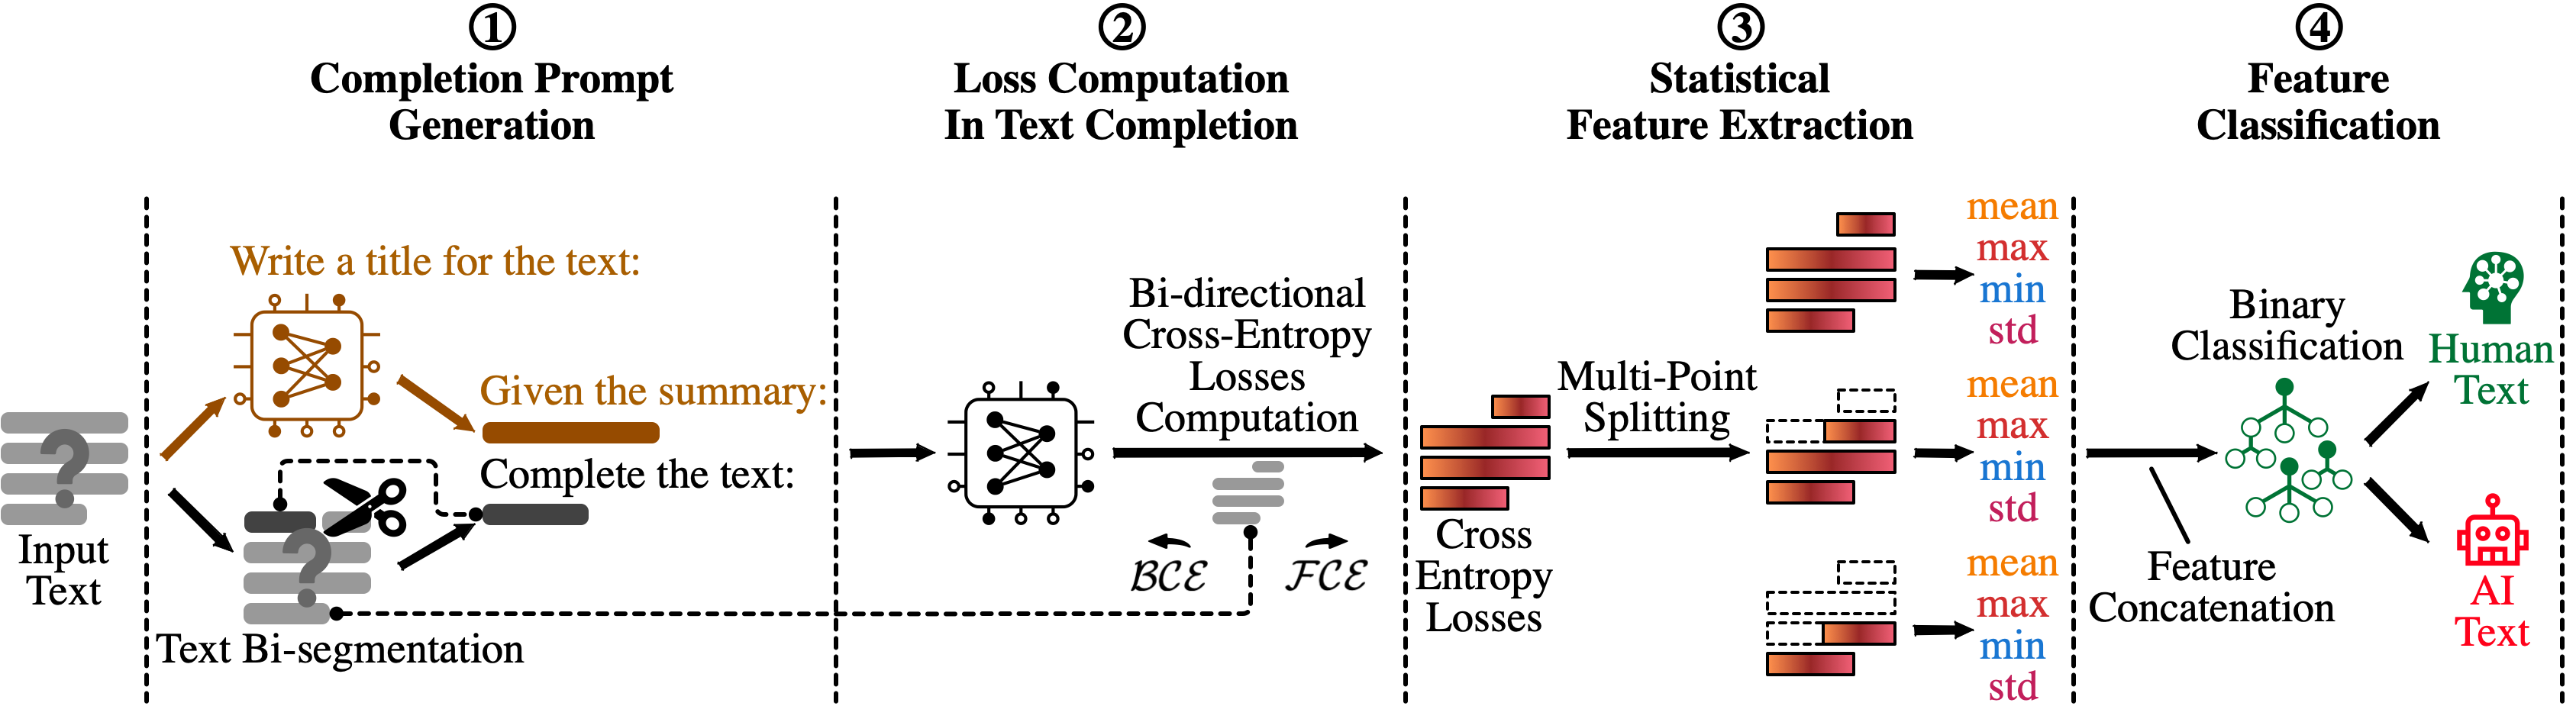
\includegraphics[width=1\textwidth]{img/BiScope/Overview.png}
    \caption{BiScope overview}
    \label{fig:BiScope-overview}
\end{figure}

\begin{enumerate}
    \item \textbf{Completion-prompt construction:} an LLM first summarizes the 
    text to obtain global context. The original text is then split in two (prefix and suffix). 
    A completion request with the summary of the text and the first part (prefix).
    \item \textbf{Loss computation:} Using the prompt, the surrogate model processes 
    the suffix text and computes two per-token cross-entropy losses:

    \begin{enumerate}
        \item \textit{Forward Cross-Entropy (FCE)}:
        the cross-entropy loss between the ground truth (suffix) next token and the LLM next token prediction given the previous tokens.
        \[
        \mathrm{FCE}_i \;=\; - \sum_{z=1}^{\lVert V \rVert} \,\tilde{P}^{\,z}_{\,i+1}\,\log\!\big(P^{\,z}_{\,i}\big),
        \]

        \item \textit{Backward Cross-Entropy (BCE)}: 
        the cross-entropy loss between the ground truth (suffix) last token and the LLM next token prediction given the previous tokens (last ground truth token included).
        \[
        \mathrm{BCE}_i \;=\; - \sum_{z=1}^{\lVert V \rVert} \tilde{P}^{\,z}_{\,i}\,\log\!\big(P^{\,z}_{\,i}\big).
        \]
    \end{enumerate}
    \begin{itemize}
        \item $V$: as vocabulary; $\lVert V\rVert$ is its size.
        \item $i$: as current position in the \emph{suffix} given the prompt+prefix (FCE valid only if $i{+}1$ exists).
        \item $z$: as index over vocabulary items $1,\dots,\lVert V\rVert$.
        \item $P^{z}_{i}$: as softmax probability assigned by the LLM at position $i$ to token $z$ given all preceding tokens up to $i$.
        \item $\tilde{P}^{z}_{i}$: as one-hot encoding of the ground-truth token at position $i$ ($\tilde{P}^{z^\star}_{i}{=}1$ if $z{=}z^\star$, else $0$).
    \end{itemize}
    \item \textbf{Feature extraction:} The text is divided into segments. 
    For each segment, statistics of FCE and BCE are 
    collected: mean, max, min, and standard deviation.

    \item \textbf{Feature classification:} All statistics are concatenated into a 
    single feature vector used to train a binary classifier that decides 
    whether the text is human- or AI-written \textit{(implemented with a Random Forest)}.
\end{enumerate}

Analysing the method, it is seen that many variables exist, such as: 
which LLM to use for completion, into how many sections to split 
the text, whether to give more or less importance to FCE and BCE. 
All these variables were not specified in the CodeMirage paper. 
For this reason, each hyperparameter was set to its default value.

\subsubsection{BiScope-improved}
This method is proposed for the first time in this thesis and attempts to modify BiScope specifically for code.
The big changes are: erase the phase of summarizing the code and the LLM used
in FCE and BCE computation.

\begin{figure}[H]
    \centering
    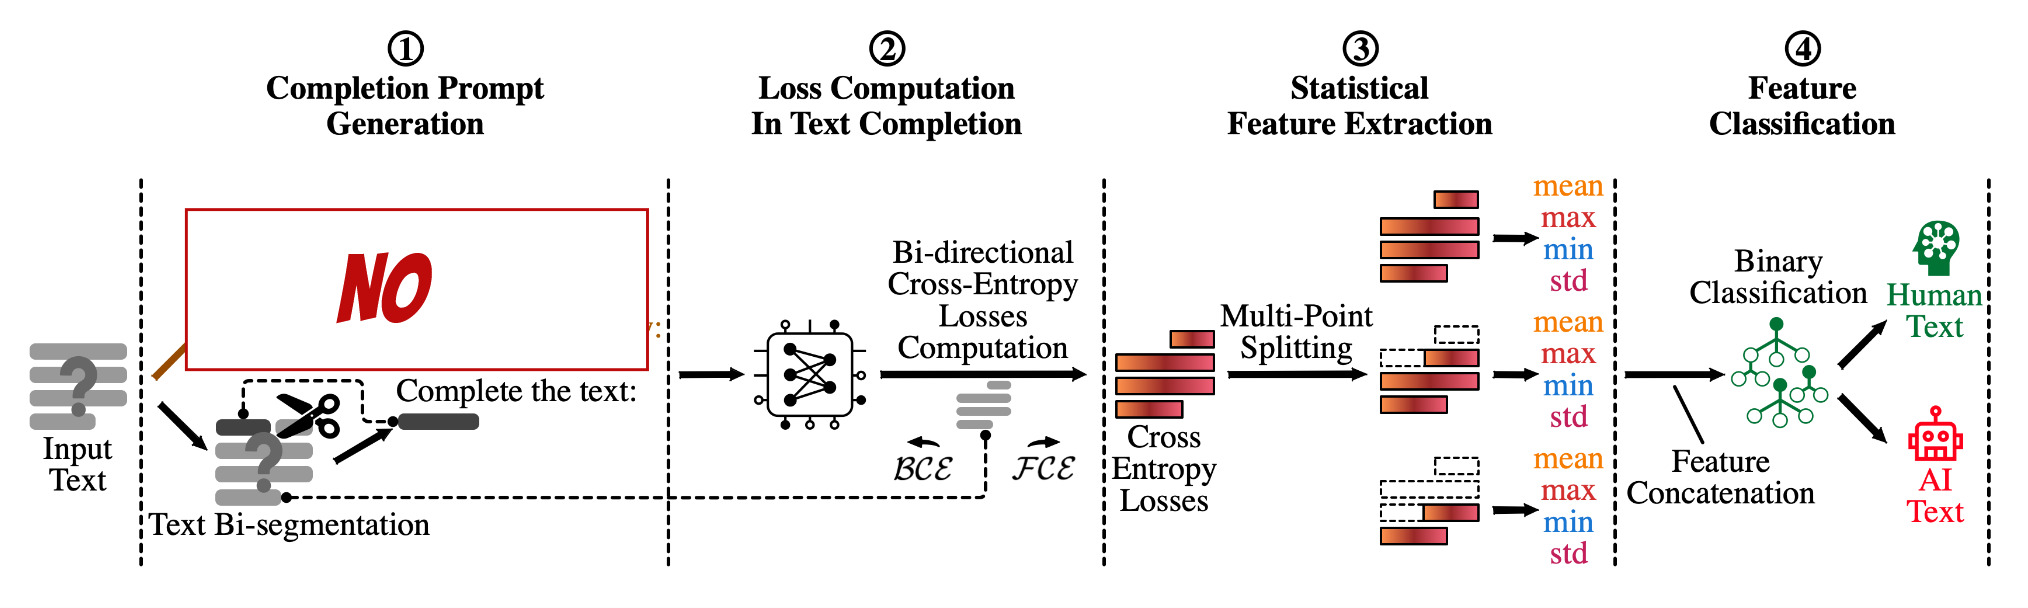
\includegraphics[width=1\textwidth]{img/BiScope/overview improved.jpg}
    \caption{BiScope overview improved}
    \label{fig:BiScope-overview-improved}
\end{figure}

The \textbf{phase of summarizing} is real useful for natural text, like chose
a title for the text (another type of prompt recommended by the authors).
The problem is that more or less every LLM can generate a good summary of
natural text, but non every LLM-code-finetuned can generate a good summary 
(or explanation) of code.
For this reason in the BiScope-improved version the summarization 
phase was removed, and we can demonstrate that it is not necessary for
achieve good results.
Erasing the summarization phase also has the advantage of speeding up
the inference phase, which is already quite slow due to the need to
perform double cross-entropy computation (BCE and FCE).

Regarding the \textbf{choice of the LLM}, 
by analysing the LLMs proposed by BISCOPE (and probably also used in the 
CodeMirage tests) on which to evaluate the loss values, it was evident 
that none of those LLMs had been fine-tuned on code:

\begin{table}[ht]
\centering
\begin{tabular}{|p{0.5\textwidth}|p{0.5\textwidth}|}
\hline
\textbf{LLM proposed} & \textbf{Code finetuning?}  \\
\hline
\textbf{Llama-2-7B\cite{touvron2023llama},Llama-2-13B\cite{touvron2023llama}, Llama-3-8B\cite{dubey2024llama}} & No  \\
\hline
\textbf{Gemma-2B\cite{team2024gemma}, Gemma-7B\cite{team2024gemma}} & Code partly present in the training dataset \\
\hline
\textbf{Mistral-7B\cite{jiang2023mistral}} & Code partly present in the training dataset  \\
\hline
\end{tabular}
\caption{Model Comparison and Training on Code}
\label{tab:modelli_codice}
\end{table}

For this reason, a retraining of the classification head was 
performed using \textbf{CodeLlama-7b-hf} \cite{roziere2023code} as the LLM.
It was chosen as the LLM because: it is not among the LLMs that generated 
code in the CodeMirage dataset; it has been fine-tuned on code in several 
languages (Python, C++, Java, PHP, TypeScript, JavaScript, C\#); it has been 
trained to respond to completion requests (required by BiScope); and it is an 
instruct version, as expected by the BiScope framework.

To evaluate the improvements introduced by changing the LLM, in-domain 
tests were conducted on the CodeMirage dataset.
\begin{figure}[H]
    \centering
    \begin{subfigure}[b]{0.45\textwidth}
        \centering
        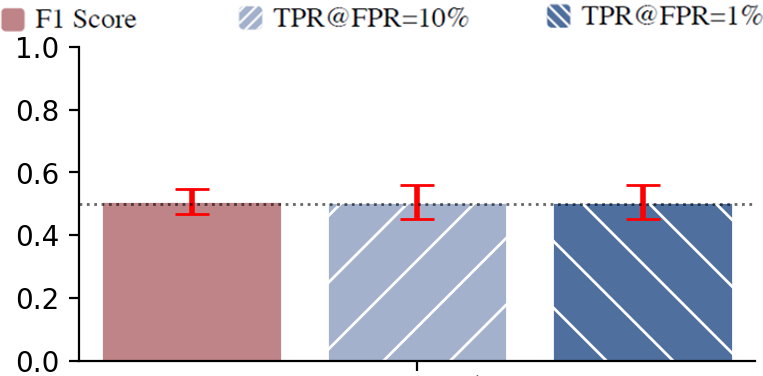
\includegraphics[width=\linewidth]{img/BiScope/standard/CodemirageOverCodemirage.png}
        \caption{BiScope standard.}
        \label{fig:BiScope standard.}
    \end{subfigure}
    \hfill
    \begin{subfigure}[b]{0.45\textwidth}
        \centering
        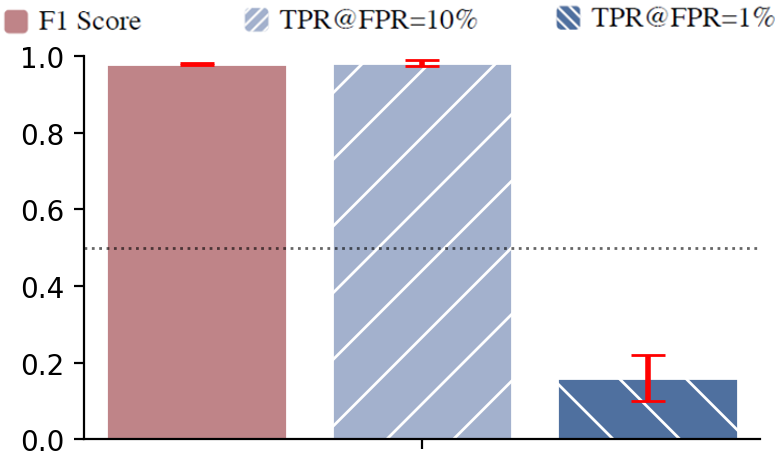
\includegraphics[width=\linewidth]{img/BiScope/test_noramle_migliorato.png}
        \caption{BiScope CodeLlama-7b-hf.}
        \label{fig:BiScope CodeLlama-7b-hf.}
    \end{subfigure}
    \caption{BiScope and BiScope improved CodeMirage in-domain test.}
    \label{fig:BiScope and BiScope improved CodeMirage in-domain test.}
\end{figure}

It is evident that the results are more than excellent. Inspecting the plot, 
it appears that with an FPR of 10\% the model attains an almost perfect TPR. 
It can also be noted that at FPR = 1\% the TPR decreases by a non-negligible 
amount. This means that, under these conditions, the model is usable only by 
accepting an error probability of about 10\% or slightly less.

\subsubsection{GPTSniffer-CodeT5+ multilingual}
This method is based on another work, GPTSniffer\cite{nguyen2024gptsniffer}, 
with the only difference 
of using a different encoder-only model. This also shows how the same methods 
can obtain extremely different results (see the TPR results at FPR = 1\% 
reported by CodeMirage \ref{fig:CodeMirage-tests}) 
without changing the methodological aspect but only by 
changing the transformer used. This should not be surprising, since much of the 
work is carried out by these networks, but it also shows how the results of the 
same method can vary greatly when a different transformer is used.

The GPTSniffer technique is based on two principles:
\begin{figure}[H]
    \centering
    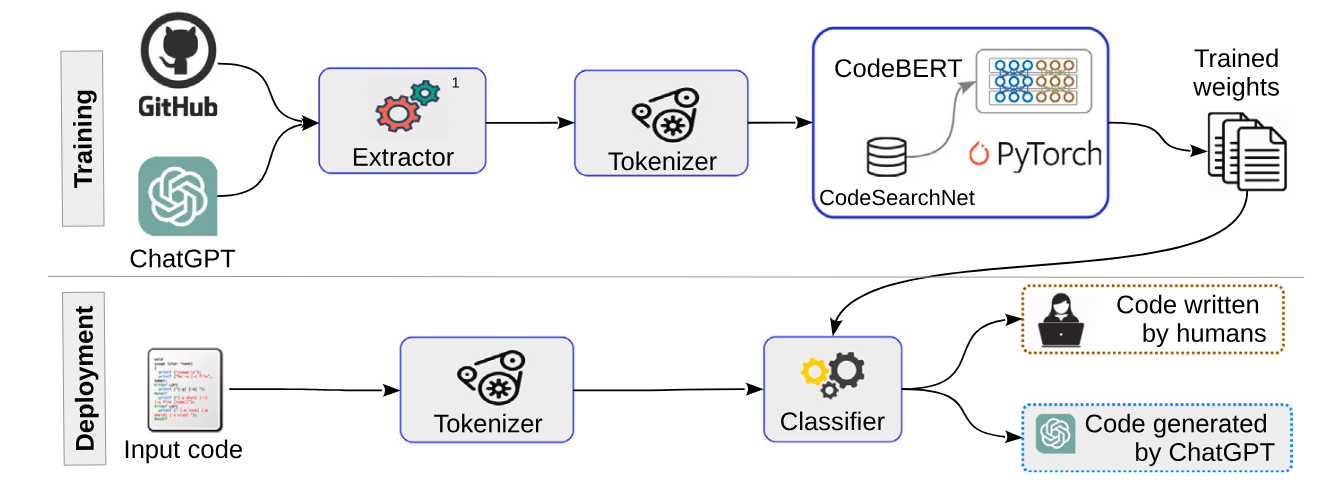
\includegraphics[width=1\textwidth]{img/gptsniffer/system components.png}
    \caption{GPTSniffer system}
    \label{fig:GPTSniffer system}
\end{figure}
\begin{enumerate}
    \item Train the transformer and the classification head on code style, 
    not on the code itself. 
    They seek to obtain this result by applying heavy preprocessing that:   
    \begin{enumerate}
        \item Removal of all imports
        \item Removal of comments
        \item Removal of formatting characters
        \item Replacement of class name
    \end{enumerate}
    \item Fine-tune the encoder-only module to obtain the best embedding 
    representation to be classified by the head.
\end{enumerate}

Unlike CodeMirage, to carry out these tests a \textbf{preprocessing 
version applicable to many programming languages} (all those present in 
the CodeMirage dataset) was developed. In fact, GPTSniffer focuses only on 
Python, which would be a problem both during training and during testing on 
a multilingual dataset.

To evaluate the improvements introduced by changing the LLM, in-domain tests 
were conducted on the CodeMirage dataset.
\begin{figure}[H]
    \centering
    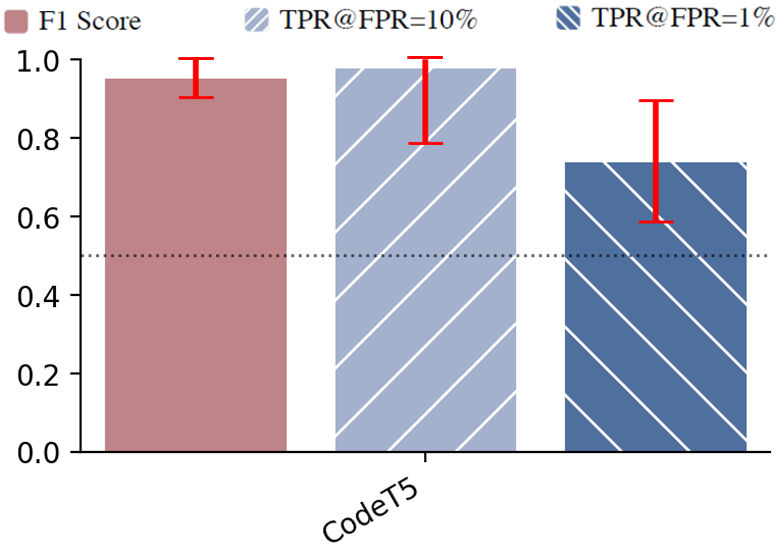
\includegraphics[width=0.8\textwidth]{img/CodeT5/default.png}
    \caption{CodeT5 tests with multilingual preprocessing CodeMirage in-domain test.}
    \label{fig:CodeT5 tests with multilingual preprocessing}
\end{figure}

Excellent performance is observed here as well. Compared with BiScope 
with CodeLlama, performance across languages remains much more variable 
(higher standard deviation). Nevertheless, very good TPR is obtained at FPR = 1\%, 
a result that is interesting and useful for scenarios where avoiding unjust 
accusations is required.



\subsubsection{UncoveringLLM}
This method was one of the first proposed for detection specifically on code. 
After recognizing that the problem on code was profoundly more complex than on 
human code, a new technique was implemented. Unfortunately, it should be noted 
that the provided repository was wholly insufficient. For this reason, the entire 
technique they proposed was reproduced from scratch.
The technique is based on a key observation: when an LLM rewrites code it previously 
generated, the differences between the two versions are minimal. Conversely, if the 
LLM rewrites code written by a human, the differences are much more significant. 
Leveraging this intuition, the detector operates in three fundamental steps:

\begin{enumerate}
\item \textbf{Rewrite the code:} An LLM is used to rewrite the code snippet under analysis. 
The model is instructed to explain the code’s functionality and rewrite it, a 
method based on chain-of-thought prompting.

\item \textbf{Measure similarity:} A code-similarity model, such as 
GraphCodeBERT\cite{guo2020graphcodebert} 
(trained with self-supervised contrastive learning), computes a similarity 
score between the original code and its rewritten version. The framework is 
flexible and not tied to a specific similarity model.

\item \textbf{Compute the detection score:} The rewriting process is repeated multiple times 
(m times), and the final similarity score is the mean of the scores from each 
rewrite. If the score exceeds a threshold, the code is classified as LLM-generated. 
According to experiments, only four rewrites are sufficient to achieve excellent results.
\end{enumerate}

The method, although interesting, presents a major problem in use: 
at least two rewrites are required for each code snippet, greatly 
lengthening both the training and inference phases. For this reason, 
despite the work recommending 4 rewrites for higher performance, the tests 
will use two rewrites, which according to the original paper’s tests does not 
reduce the F1-score by more than 0.1.

To use this method, the previously described framework~\ref{section:Test framework} 
was therefore used (with slight modifications) to generate code rewrites on a 
dataset. In this way it was possible to run tests on the various available datasets.

It is important to note that, since CodeBERT was not retrained for the tests 
conducted on this method, the model used to rewrite the code is one of those 
adopted during CodeBERT’s training 
(\href{https://huggingface.co/codellama/CodeLlama-13b-Instruct-hf}{CodeLlama-13-Instruct}\cite{roziere2023code}).

\begin{figure}[H]
    \centering
    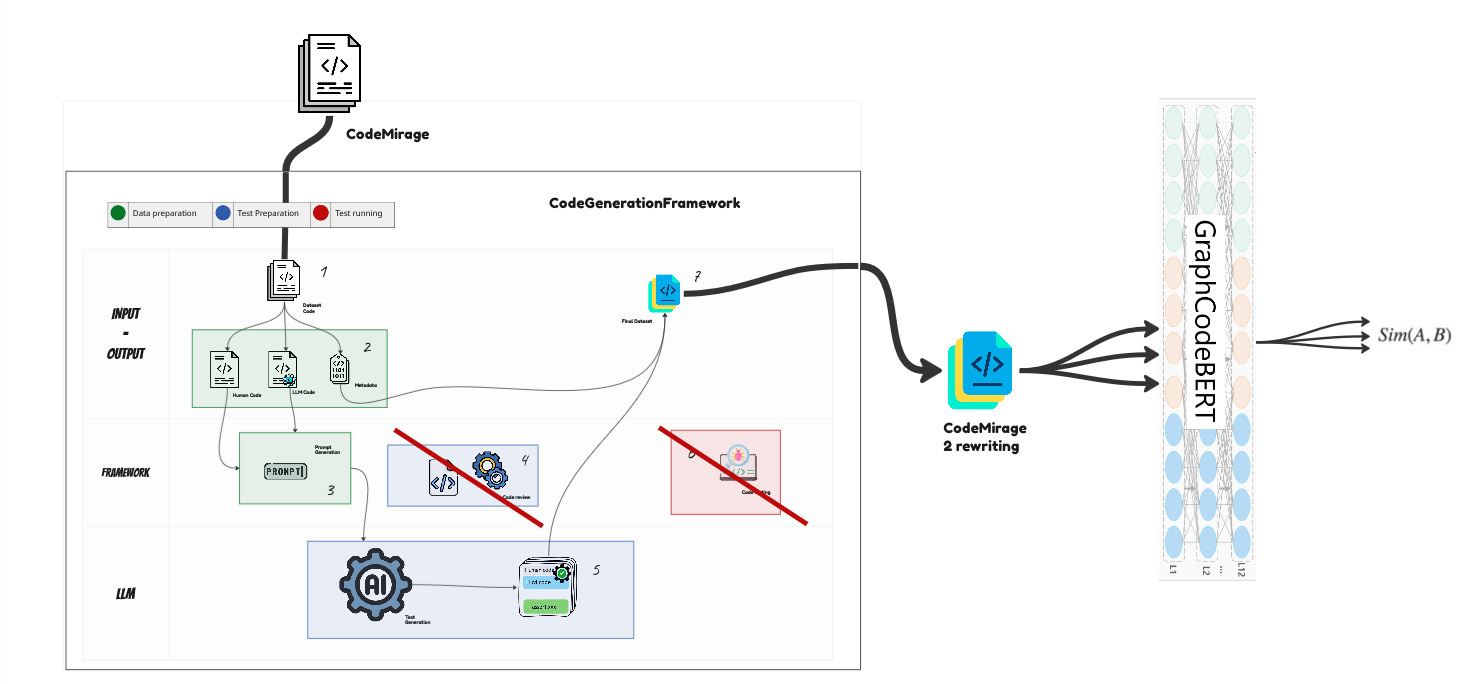
\includegraphics[width=1\textwidth]{img/UncoveringLLM/framework.jpg}
    \caption{UncoveringLLM Framework}
    \label{fig:UncoveringLLM Framework}
\end{figure}




\subsubsection{LLMPPL}
The work “Detecting AI-Generated Code Assignments Using Perplexity 
of Large Language Models” proposes a zero-shot detection method based 
on perplexity. However, from their official repository on 
\href{https://github.com/Arrtourz/llmppl}{GitHub} 
it can be seen that only the code for computing perplexity was released, 
and not the code for all the subsequent evaluations described in their 
work. Nevertheless, it is appropriate to test what was implemented. 
In this work, perplexity is computed using different techniques, 
including the use of a \textbf{Mamba model}. 
In particular, they implemented the calculation of 
perplexity with \href{https://huggingface.co/state-spaces/mamba-130m-hf}{mamba-130m-hf}
The use of Mamba for perplexity 
calculation is very interesting, since it is known that Mamba models 
tend to be much more efficient than transformers 
(linear-time computation rather than exponential).

Quickly repeating how the perplexity score is computed in general:
\begin{enumerate}
    \item \textbf{Tokenization} \\
    A text sequence is converted into token IDs, where $s$ is the text:
    \[
        T(s) = (x_1, \dots x_L), \quad  x_i \in V = {1, \dots, n}
    \]

    \item \textbf{Autoregressive prediction} \\
    The model produces logits for each position $i$ given the prefix, 
    where $|V|$ is the vocabulary size and $f_M$ is the 
    LLM \textit{(or in this case the mamba model)}:
    \[
        Z_i = f_M(x_{0:i-1}), \quad Z_i \in \mathbb{R}^{|V|}
    \]

    \item \textbf{Token probabilities} \\
    Apply the softmax function to obtain probabilities:
    \[
        Y_i=\mathrm{softmax}(Z_i), \quad
        Y_{ij}=P(v_j \mid x_{0:i-1})=\frac{\exp(Z_{ij})}{\sum_{u\in V}\exp(Z_{iu})}.
    \]

    \item \textbf{Shifted targets} \\
    For causal LM, the target at step $i$ is the next token in the sequence:
    \[
        \text{target at } i \text{ is } x_i \text{ given } x_{0:i-1}, \quad i=1,\dots,L.
    \]

    \item \textbf{Negative log-likelihood per token} \\
    \[
        \mathrm{NLL}_i = -\log Y_{i\,x_i}.
    \]

    \item \textbf{Average loss (cross-entropy in nats)} \\
    \[
        \mathrm{loss}=\frac{1}{L}\sum_{i=1}^{L}\mathrm{NLL}_i
        =-\frac{1}{L}\sum_{i=1}^{L}\log Y_{i\,x_i}
        =\log\mathrm{PPL}_M(s).
    \]

    \item \textbf{Perplexity} \\
    So more the perplexity is low, more the text is likely to be generated by an LLM:
    \[
        \mathrm{PPL}_M(s)=\exp(\mathrm{loss}).
    \]
\end{enumerate}

In order to select the best perplexity threshold, 
a CoDet-M4\ref{section:CoDet-M4} sub-dataset was used, and the threshold that 
maximized TPR/FPR was set.


\begin{figure}[H]
    \centering
    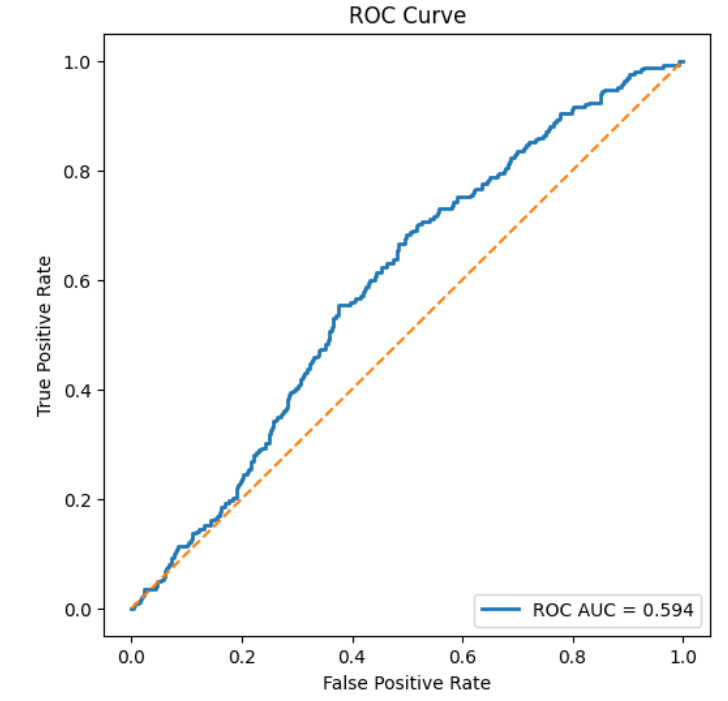
\includegraphics[width=0.6\textwidth]{img/LLMPPL/AUC.png}
    \caption{MAX TPR/FPR used to select the threshold.}
    \label{fig:TPR/FPR used to select the threshold.}
\end{figure}



\subsubsection{Binoculars}
\newcommand{\PPL}{\mathrm{PPL}}
\newcommand{\xPPL}{\mathrm{xPPL}}
Classical detection methods rely mainly on PPL calculation. 
Binoculars takes a step further, pointing out that a text may 
have low PPL even if generated by an LLM with a particular prompt. 
It is well known that there is an entire field called prompt 
engineering that focuses precisely on obtaining certain results 
from an LLM by simply changing the prompt. Since the prompt is so 
fundamental during generation, it cannot be ignored in PPL calculation. 
However, it is obviously not possible to recover the prompt given only 
the generated text (in this case, the code). For this reason, 
Binoculars proposes evaluating the value 
B, given by the ratio between the PPL computed by a first LLM and the PPL of a second LLM on the predictions of the first LLM.

PPL over first LLM:
\[
\log \PPL_{M_1}(s)
= -\frac{1}{L}\sum_{i=1}^{L}\log p_{M_1}(x_i\mid x_{<i}).
\]

PPL over second LLM of the predictions of the first LLM:
\[
\log \xPPL_{M_1,M_2}(s)
= -\frac{1}{L}\sum_{i=1}^{L}\sum_{v\in V}
p_{M_2}(v\mid x_{<i})\,\log p_{M_1}(v\mid x_{<i}).
\]

Ratio:
\[
B_{M_1,M_2}(s)=\frac{\log \PPL_{M_1}(s)}{\log \xPPL_{M_1,M_2}(s)}.
\]

Deduction:
\begin{itemize}
\item LLM-like text: $\PPL_{M_1}(s)\approx \xPPL_{M_1,M_2}(s)\ \Rightarrow\ B$ small.
\item Human-like text: $\PPL_{M_1}(s)\gg \xPPL_{M_1,M_2}(s)\ \Rightarrow\ B$ large.
\item Assumption needed: $M_1$ and $M_2$ are similar (same tokenizer and comparable strength).
\end{itemize}
The calculation of PPL by the second LLM on the predictions of 
the first is intended to “normalize” the perplexity value due to 
the particularity of the generated text (in this case code) and thus 
the particularity of the prompt. It is easy to see that this issue 
is more evident in natural-language texts; nevertheless, this 
method was also tested using LLMs fine-tuned on code, in particular 
\href{https://huggingface.co/meta-llama/CodeLlama-7b-hf}
{meta-llama/CodeLlama-7b-hf} as the first LLM and 
\href{https://huggingface.co/meta-llama/CodeLlama-7b-Instruct-hf}{CodeLlama-7b-Instruct-hf} 
\cite{roziere2023code} as the second LLM.
Tests were also conducted with the LLMs used in the original work:
\href{https://huggingface.co/tiiuae/falcon-7b}{falcon-7b} and 
\href{https://huggingface.co/tiiuae/falcon-7b-instruct}{falcon-7b-instruct}
\cite{falcon40b}








%%%%%%%%%%%%%%%%%%%%%%%%%%%%%%%%%%%%%%%%%%%%%%%%%%%%%%%%%%%%%%%%%%
\clearpage
\subsection{Tests}
\subsubsection{Out-Of- Domain tests}
In this testing phase, the methods are evaluated on 
CodeMirage but were trained on a different dataset 
(CoDet for BiScope and GPTSniffer; the UncoveringLLM 
model was not retrained; Mamba perplexity and Binoculars 
do not require training). These tests are useful both for 
assessing out-of-domain performance and for making qualitative 
considerations about the ability of the method to generalize 
LLM code characteristics. If a method shows high accuracy on 
an LLM seen during training but extremely low accuracy on 
unseen LLMs, it can be concluded that the method is poorly 
generalizable. If instead the performance remains roughly 
the same across different LLMs, it can be concluded that 
the detection method does not learn the “style” of a 
specific LLM but intrinsic characteristics of code 
generation through transformers.


\begin{figure}[H]
    \centering
    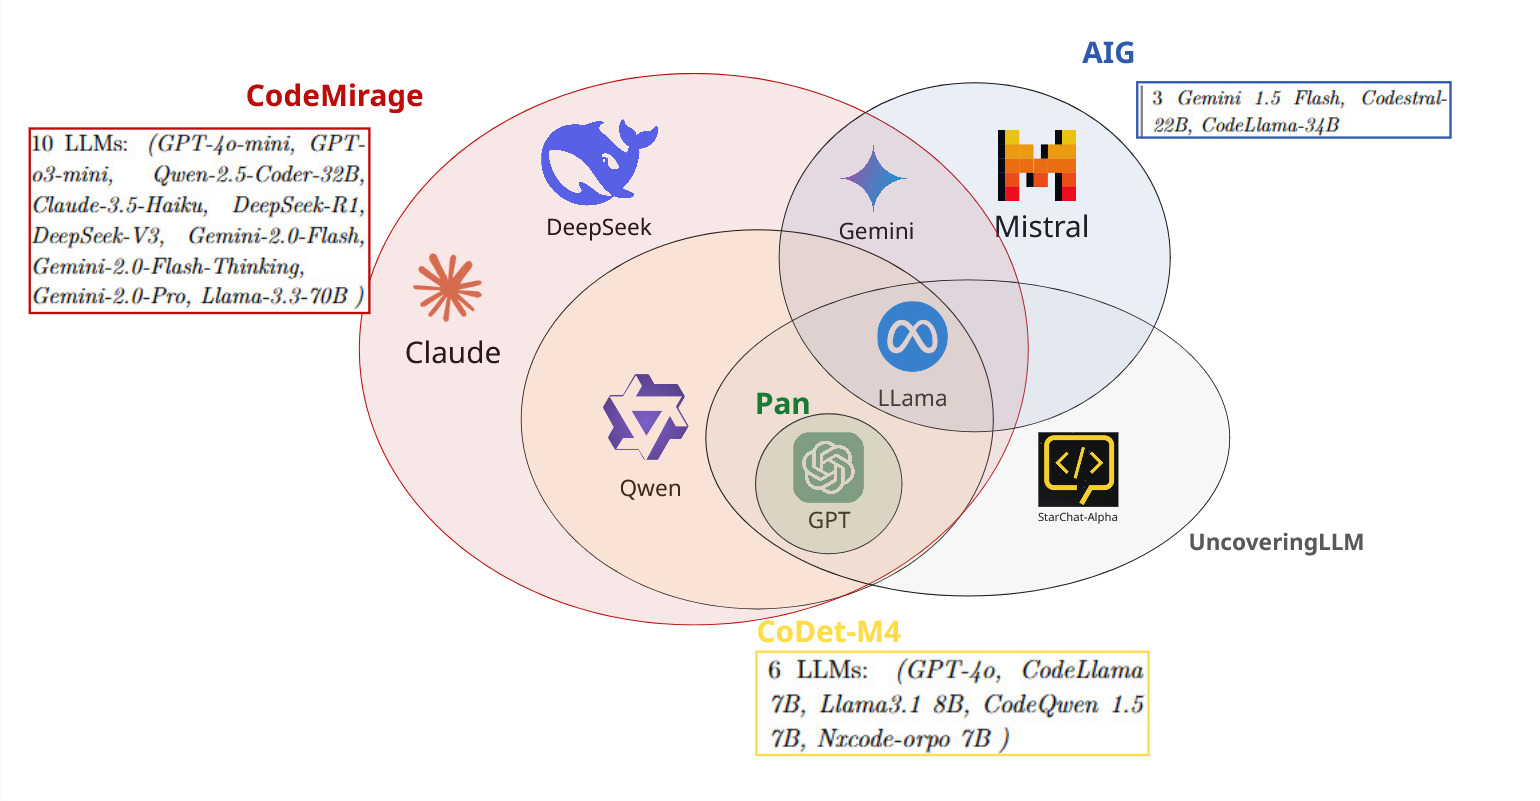
\includegraphics[width=1\textwidth]{img/1/Untitled - LLM over dataset.jpg}
    \caption{The different LLMs familys inside the datasets.}
    \label{fig:LLMOverDataset}
\end{figure}



\subsubsection{BiScope-improved}

\begin{figure}[H]
    \centering
    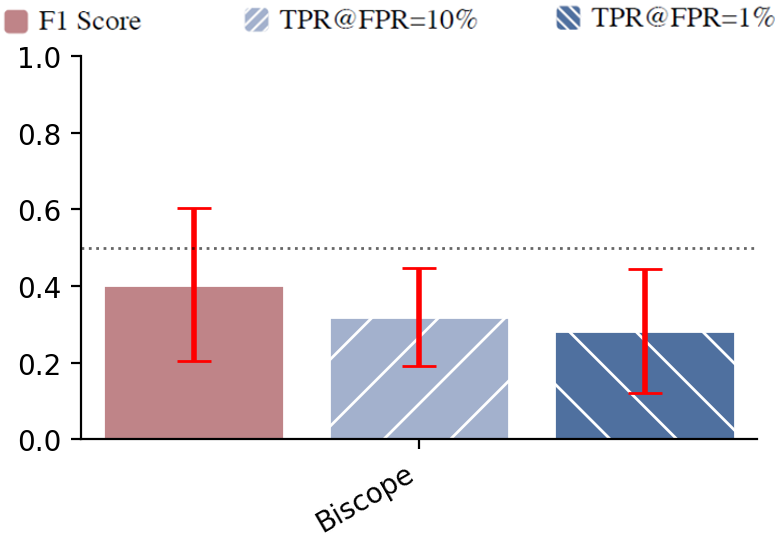
\includegraphics[width=0.6\textwidth]{img/TEST/BiScope/fromCodetCodemirange/test_noramle_migliorato-Recuperato.png}
    \caption{BiScope. Learning:Codet Test:Codemirange}
    \label{fig:BiScope1}
\end{figure}

\begin{figure}[H]
    \centering
    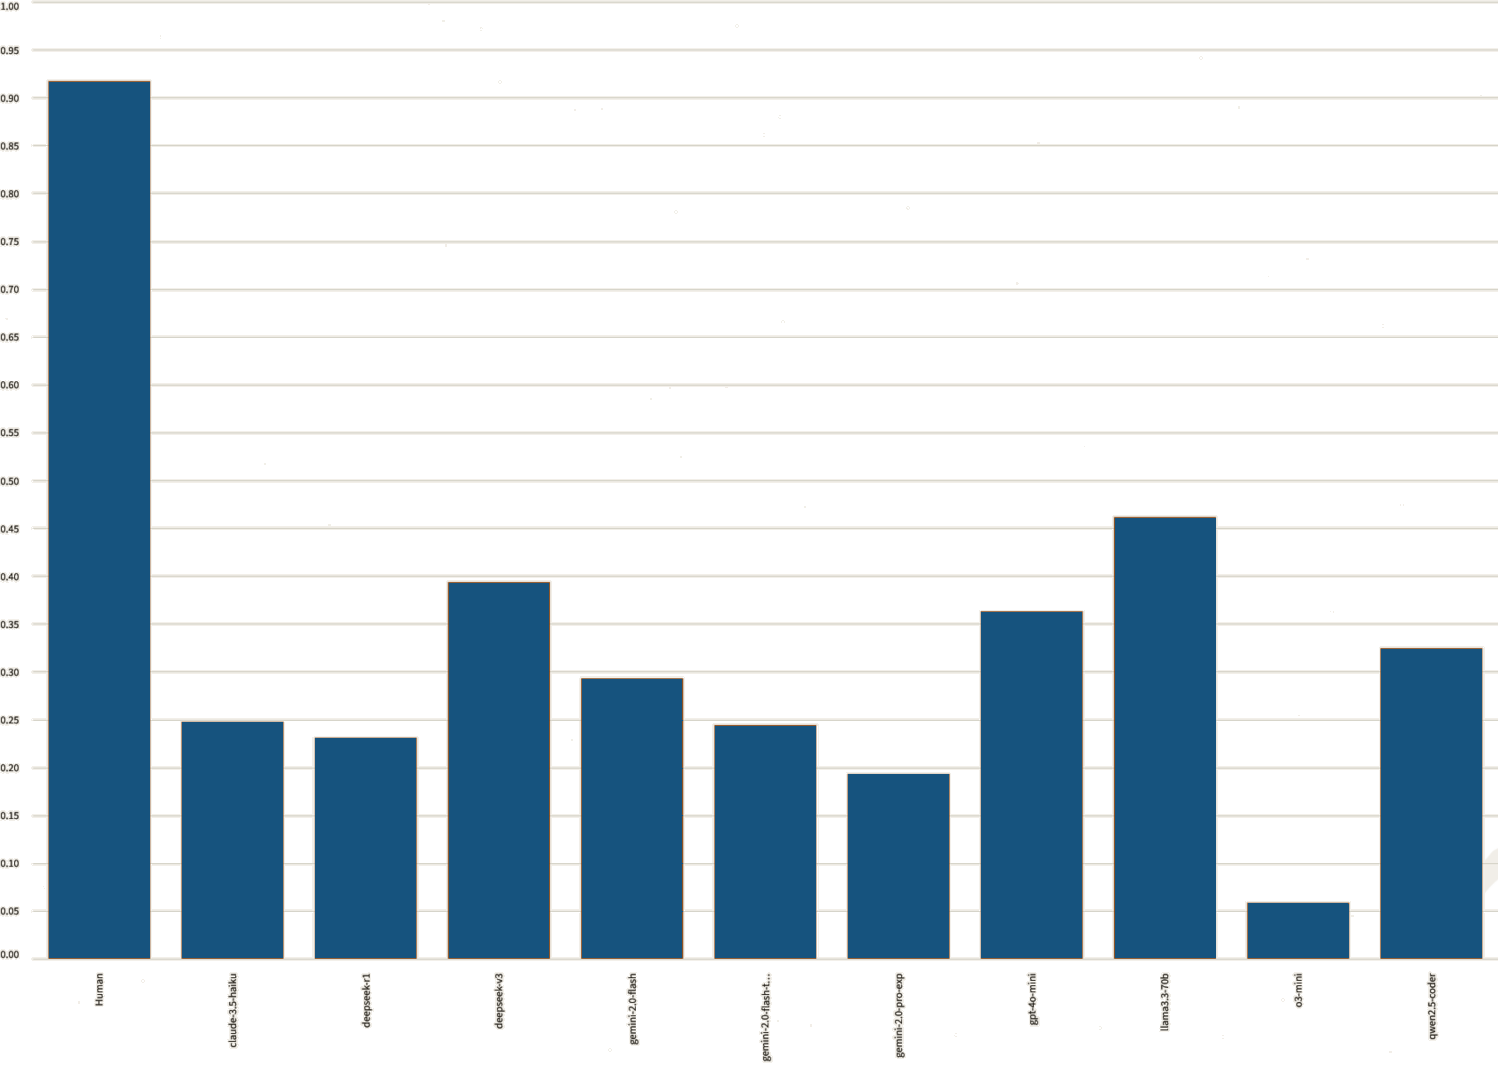
\includegraphics[width=0.6\textwidth]{img/TEST/BiScope/fromCodetCodemirange/accuracy LLM (2).png}
    \caption{BiScope. Learning:Codet Test:Codemirange Accuracy over LLMs}
    \label{fig:BiScope1accLLM}
\end{figure}

\subsubsection{GPTSniffer-CodeT5+ multilingual}



\subsubsection{UncoveringLLM}




\subsubsection{LLMPL}





\subsubsection{Binoculars}



%%%%
\subsection{AIGCode test}


\subsubsection{BiScope}

\subsubsection{BiScope-improved}


\subsubsection{GPTSniffer-CodeT5+ multilingual}



\subsubsection{UncoveringLLM}




\subsubsection{LLMPL}



\subsubsection{Binoculars}